\documentclass{standalone}
\usepackage{tikz}
\usepackage{tikz-qtree}
\usepackage[makeroom]{cancel}
\usetikzlibrary{fit}


\begin{document} 
	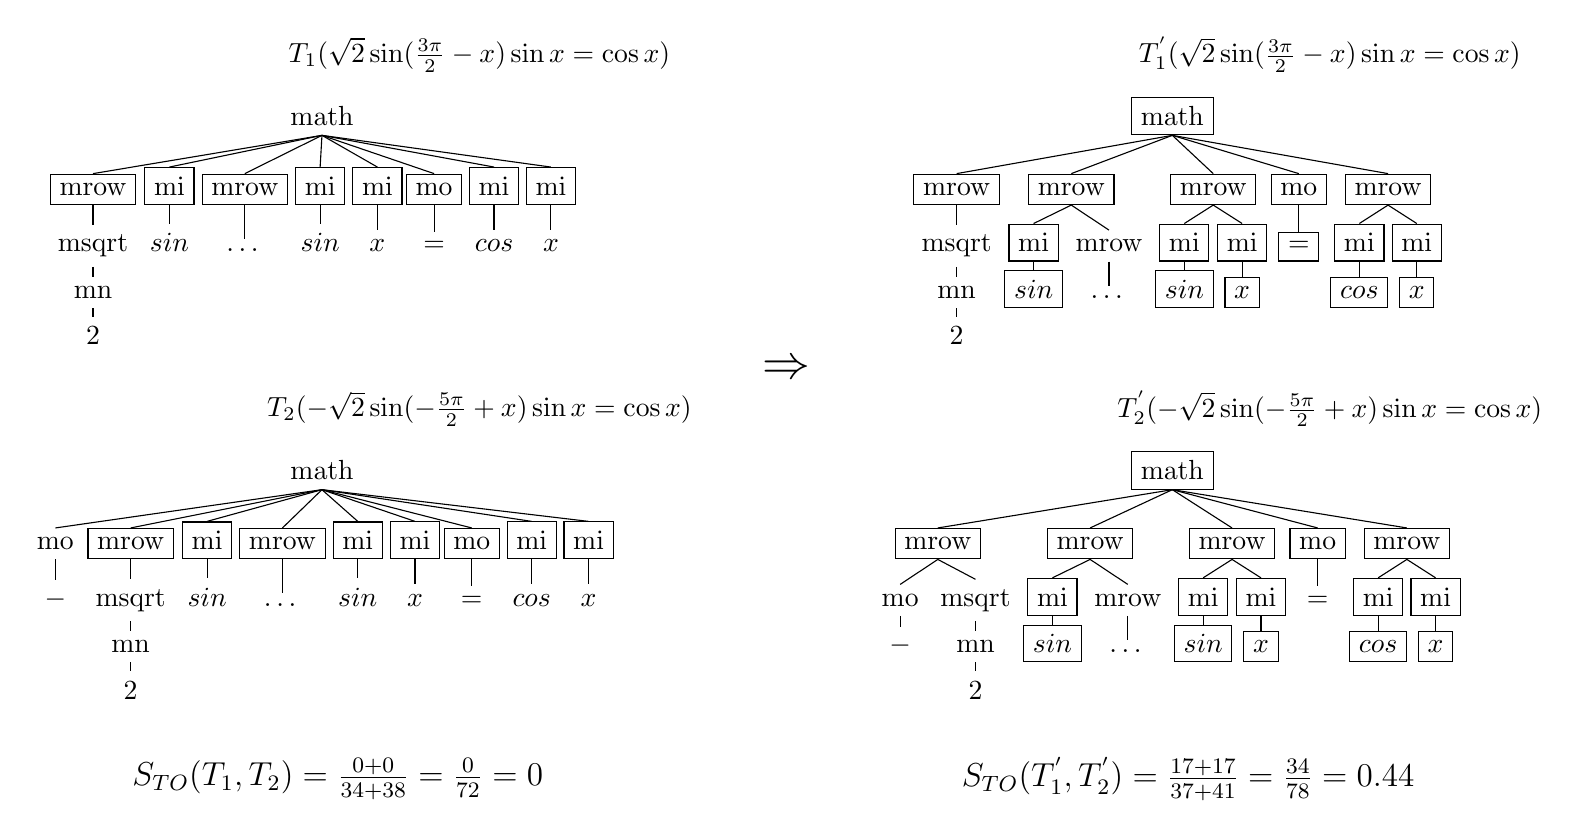
\begin{tikzpicture}[sibling distance=1.2pt]
	\tikzset{level 1/.style={level distance=2.1\baselineskip}}
	\tikzset{level 2/.style={level distance=1.7\baselineskip}}
	\tikzset{level 3+/.style={level distance=1.4\baselineskip}}
	\node (x) at (5.9,-3.1) {\LARGE{$\Rightarrow$}};

	    \node (x) at (2.0,0.9) {$T_1(\sqrt{2}\sin (\frac{3\pi}{2} - x)\sin x = \cos x)$};
	    \Tree [.\node[]{math};
	    		[.\node[draw]{mrow}; 
	    			[.\node[]{msqrt}; 
	    				[.\node[]{mn};
	    					[.\node[]{$2$}; ]
	    				]
	    			]
	    		]
	    		[.\node[draw]{mi}; \node[]{$sin$}; ]
	    		[.\node[draw](m2){mrow}; \node[]{\dots}; ]
	    		[.\node[draw]{mi}; \node[]{$sin$}; ]
	    		[.\node[draw]{mi}; \node[]{$x$}; ]
	    		[.\node[draw]{mo}; \node[]{$=$ };]
	    		[.\node[draw]{mi}; \node[]{$cos$}; ]
	    		[.\node[draw]{mi}; \node[]{$x$}; ]
	          ]
	    

		\begin{scope}[yshift=-4.5cm]
			\tikzset{level 1/.style={level distance=2.1\baselineskip}}
			\tikzset{level 2+/.style={level distance=1.7\baselineskip}}
		    \node (x) at (2,0.9) {$T_2(-\sqrt{2}\sin (-\frac{5\pi}{2} + x)\sin x = \cos x)$};
		    \Tree [.\node[]{math};
		    		[.\node[]{mo}; \node[]{$-$ };]
		    		[.\node[draw]{mrow};
		    			[.msqrt 
		    				[.mn
		    					[.$2$ ]
		    				]
		    			]
		    		]
		    		[.\node[draw]{mi}; \node[]{$sin$}; ]
		    		[.\node[draw]{mrow}; \node[]{\dots}; ]
		    		[.\node[draw]{mi}; \node[]{$sin$}; ]
		    		[.\node[draw]{mi}; \node[]{$x$}; ]
		    		[.\node[draw]{mo}; \node[]{$=$ };]
		    		[.\node[draw]{mi}; \node[]{$cos$}; ]
		    		[.\node[draw]{mi}; \node[]{$x$}; ]
		          ]
		          \node (x) at (0.2,-3.8) {\large{$S_{TO}(T_1, T_2) = \frac{0+0}{34+38} = \frac{0}{72} = 0$}};
		\end{scope}


		\begin{scope}[xshift=10.8cm]
			\tikzset{level 1/.style={level distance=2.1\baselineskip}}
			\tikzset{level 2/.style={level distance=1.7\baselineskip}}
			\tikzset{level 3+/.style={level distance=1.4\baselineskip}}

		    \node (x) at (2.0,0.9) {$T_1^{'}(\sqrt{2}\sin (\frac{3\pi}{2} - x)\sin x = \cos x)$};
		    \Tree [.\node[draw]{math};
		    		[.\node[draw]{mrow}; 
		    			[.msqrt 
		    				[.mn $2$ ]
		    			]
		    		]
		    		[.\node[draw]{mrow}; 
		    			[.\node[draw]{mi}; \node[draw]{$sin$}; ]
		    			[.mrow \node{\dots}; ]
		    		]
		    		[.\node[draw]{mrow}; 
		    			[.\node[draw]{mi}; \node[draw]{$sin$}; ]
		    			[.\node[draw]{mi}; \node[draw]{$x$}; ]
		    		]
		    		[.\node[draw]{mo}; \node[draw]{$=$}; ]
		    		[.\node[draw]{mrow}; 
		    			[.\node[draw]{mi}; \node[draw]{$cos$}; ]
		    			[.\node[draw]{mi}; \node[draw]{$x$}; ]
		    		]
		          ]
		\end{scope}


		\begin{scope}[xshift=10.8cm, yshift=-4.5cm]
			\tikzset{level 1/.style={level distance=2.1\baselineskip}}
			\tikzset{level 2/.style={level distance=1.7\baselineskip}}
			\tikzset{level 3+/.style={level distance=1.4\baselineskip}}

		    \node (x) at (2.0,0.9) {$T_2^{'}(-\sqrt{2}\sin (-\frac{5\pi}{2} + x)\sin x = \cos x)$};
		    \Tree [.\node[draw]{math};
		    		[.\node[draw]{mrow}; 
		    			[.mo $-$ ]
		    			[.msqrt 
		    				[.mn $2$ ]
		    			]
		    		]
		    		[.\node[draw]{mrow}; 
		    			[.\node[draw]{mi}; \node[draw]{$sin$}; ]
		    			[.mrow \node{\dots}; ]
		    		]
		    		[.\node[draw]{mrow}; 
		    			[.\node[draw]{mi}; \node[draw]{$sin$}; ]
		    			[.\node[draw]{mi}; \node[draw]{$x$}; ]
		    		]
		    		[.\node[draw]{mo}; $=$ ]
		    		[.\node[draw]{mrow}; 
		    			[.\node[draw]{mi}; \node[draw]{$cos$}; ]
		    			[.\node[draw]{mi}; \node[draw]{$x$}; ]
		    		]
		          ]
		          \node (x) at (0.2,-3.8) {\large{$S_{TO}(T_1^{'}, T_2^{'}) = \frac{17 + 17}{37 + 41} = \frac{34}{78} = 0.44$}};
		\end{scope}


	\end{tikzpicture}
\end{document} 